\documentclass{../template/Preport}

\usepackage{hyperref}
\hypersetup{
    colorlinks=true,
}

\exname{声速的测定} %实验名称
\instructor{刘振武} %指导教师
\class{周三上午} %班级
\name{何铭源} %姓名
\stuid{3240104481} %学号

\nyear{2025} %年
\nmonth{9} %月
\nday{24} %日
\nweekday{三} %星期几

\begin{document}
\makeatletter
\renewcommand{\figurename}{图}
\renewcommand{\tablename}{表}
\setcounter{page}{0}
\makecover

\section{预习报告(10分)}
\subsection{实验综述(5分)}
\subsubsection{实验目的}
\begin{enumerate}
	\item 了解声波的特性,加深对振动合成和波干涉理论的理解
	\item 学会用相位差法和驻波法测定声速在空气中的传播速度
	\item 学习示波器和信号发生器的使用方法
\end{enumerate}
\subsubsection{实验原理}
\begin{enumerate}
    \item 超声波传播速度:声波在理想气体中传播可看作绝热过程,其传播速度$V=\sqrt{\frac{\gamma RT}{M}}$(
    M为气体摩尔质量,R为普适气体常量,$\gamma$为热容比,T为热力学温度)。
    在0$\si{\degreeCelsius}$时,$V=331.45\si{\metre\per\second}$。在t$\si{\degreeCelsius}$时,$V_t = 331.45\sqrt{1+\frac{t}{273.15}}\si{\metre\per\second}$。
    声波在不同介质中传播速度不同。最简单的方法是直接测量声波振动的波长与频率,$V=\lambda f$。
    $f$由仪器给定,我的仅需使用驻波法(或共振干涉法)或相位比较法测定$\lambda$。
    \item 驻波法测波长:由于入射波和反射波相互叠加,两个波节之间形成共振驻波现象,波幅达到极大值。
    由于纵波的性质,振动位移处于波节时,声压处于波腹,即接收器端面移动位移为一波节时,接收到的声压最大,经接收器转换的电信号最强。驻波共振条件为:$L_n = n\frac{\lambda}{2}$ (n=1,2,3...)\\
    将接收信号输入示波器就可看到最大波振幅,
    接收端每移动距离$\Delta L$使示波器上再次观测到最大波振幅移动距离满足:$\Delta L = L_{n+1} - L_n = n\frac{\lambda}{2}$\\
    准上式代入$v=\lambda f$,即可得$v$
    \item 相位比较法测波长:沿波传播方向上的任意两点,其振动状态相同,或者说其相位差为$2\pi$的整数倍时,
    两点间距为$\lambda$的整数倍,利用这一原理可测波长。
    我们通过移动接收端改变相位差$\Delta\varphi$,使示波器上显示的李萨如图形如下变化,记录下$N$次二、三象限直线或二四象限图形位置读数$L_i$,同样有$\Delta L = L_{n+1} - L_n = \frac{\lambda}{2}$,代入$v=\lambda f$可得$v$
\end{enumerate}
\begin{figure}[H]
    \centering
    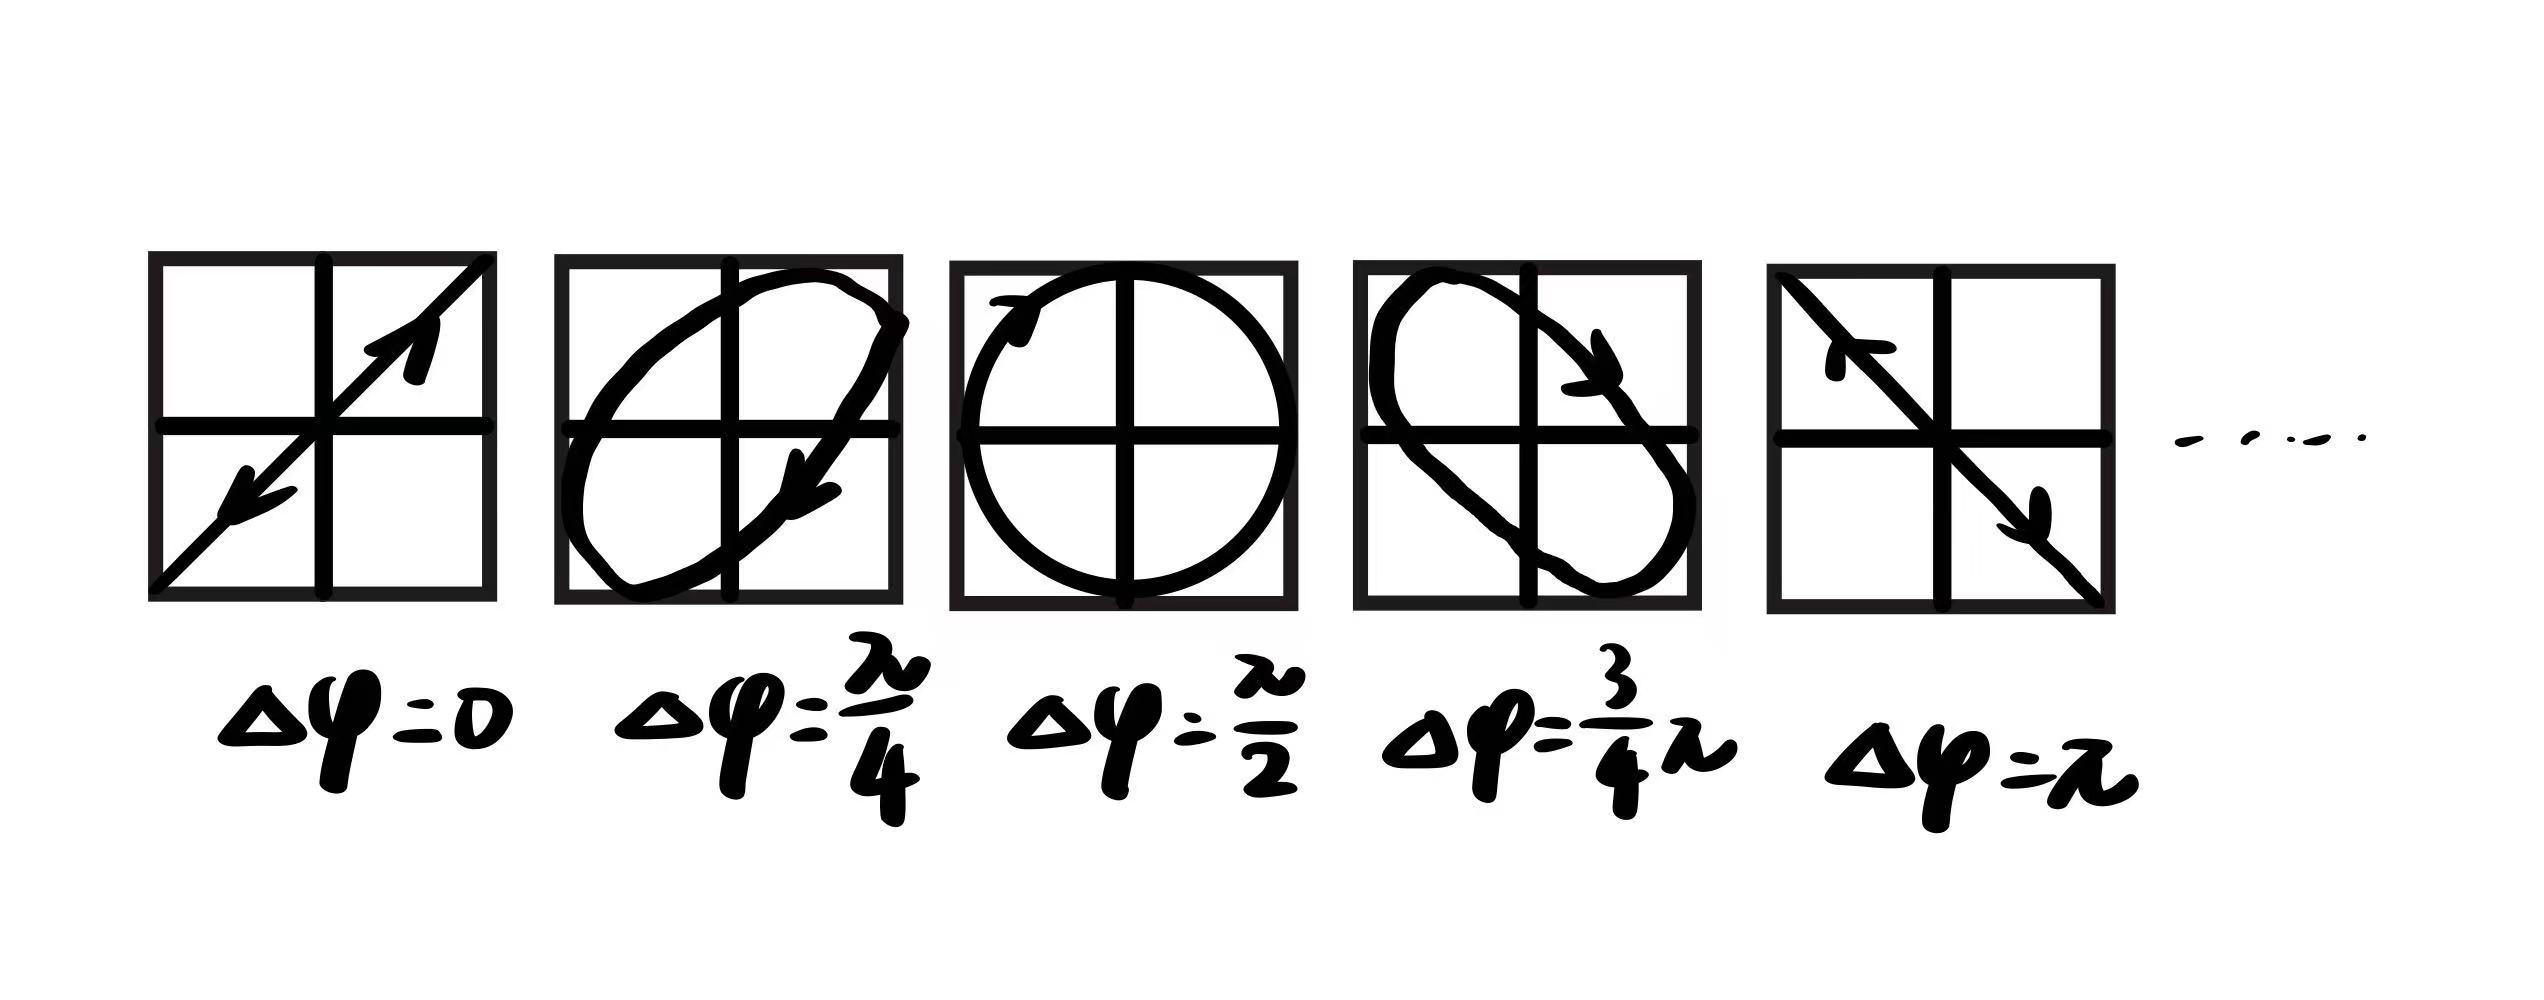
\includegraphics[width=0.8\textwidth]{figures/1.jpg}
    \caption{相位比较法测波长中的李萨如图形}
\end{figure}
\subsection{实验重点(3分)}
% (简述本实验的学习重点,不超过100字。)
\begin{enumerate}
    \item \textbf{系统调节:}实验时只有信号频率与两个具有相同固有频率的换能转换器一致时,
    同时只有发射端面与接收端面相平行时,才能保证良好的实验效果。

    \textbf{调节方法:}使移动端与固定端尽量做到并平行,将接收信号输入示波器Y轴,
    在信号发生器上调节频率旋钮选择谐振频率(约40\si{\kilo\hertz}),然后微调信号发生器的频率旋钮,
    直到示波器上出现最大振幅,此时显示的频率数值才是实验所需的谐振频率。

    \item \textbf{驻波法测声速:}调节超声换能器至最佳状态后,
    将移动接收端来回移动,观察干涉现象。缓慢移动接收端,
    示波器上出现最大振幅波形,从标尺上读得此时的位置读数$L_1$,
    继续向同一方向移动接收端,逐次记录出现最大振幅的位置$L_i$,连续记录8次,同时记下$f$。
    若显示频率有细微增减,可读记起始频率$f_1$和结束测量时$f_2$,以$\frac{f_1+f_2}{2}$作为$f$。

    \item \textbf{相位差法测声速:}将发射端的信号输入示波器X轴,
    选择发射端与接收端两振动信号分别输入示波器X和Y轴的偏转板上,在屏幕上显示了合成后的李萨如图形。
    移动接收端就可在示波器上看到一、三象限的直线,从标尺上读得此时的位置$L_1$,
    再像移动接收端,测得在示波器上看到二、四象限的直线,从标尺上读得此时位置读数$L_2$,同时记下此时$f$,连续记录8个数据。
\end{enumerate}
\subsection{实验难点(2分)}
% (简述本实验的实现难点,不超过100字。)
\begin{enumerate}
    \item \textbf{波形变化可能不明显:}尽量使移动端换能器靠近固定端,使波形变化明显。
    \item \textbf{移动接收端方向问题:}移动接收端时必须沿一方向,严禁因相位差超过需读数点而反向移动(如发生则重做实验),否则会产生误差。
    \item \textbf{读数有效位数:}读数时注意有效位数,螺旋测微仪分度值为0.01\si{\milli\metre},故包含估读的读数应到0.001\si{\milli\metre}数量级。
\end{enumerate}
{\fangsong \noindent \textbf{注意事项:}

\begin{enumerate}[label=\arabic*.]
    \item 用PDF格式上传“预习报告”,文件名:学生姓名+学号+实验名称+周次。
    \item “预习报告”必须递交在“学在浙大”本课程内对应实验项目的“作业”模块内。
    \item “预习报告”还须拷贝到“实验报告”中(以便教师批改)。
    \item “大学物理实验”课程选做实验使用本“预习报告”;必做实验无须写预习报告,前往“学在浙大”完成预习测试即可。
\end{enumerate}}
\begin{center}
    \fbfangsong{浙江大学物理实验教学中心制}
\end{center}
\end{document}
